% ============================================================
%  Fixed-point engineering via additive perturbations of the
%  logistic map: drift, stability shift, selectivity, and
%  null frequencies
%
%  Target: Physical Review E (nonlinear dynamics)
%
%  Build: pdflatex perturbation_probing
%         bibtex   perturbation_probing
%         pdflatex perturbation_probing  (x2)
% ============================================================

\documentclass[aps,pre,twocolumn,superscriptaddress,nofootinbib,
               longbibliography,floatfix]{revtex4-2}

% ---- Unicode (pdflatex + UTF-8) ----------------------------
\DeclareUnicodeCharacter{03B1}{\ensuremath{\alpha}}
\DeclareUnicodeCharacter{03B5}{\ensuremath{\varepsilon}}
\DeclareUnicodeCharacter{03C9}{\ensuremath{\omega}}
\DeclareUnicodeCharacter{03C3}{\ensuremath{\sigma}}
\DeclareUnicodeCharacter{2264}{\ensuremath{\leq}}
\DeclareUnicodeCharacter{2265}{\ensuremath{\geq}}
\DeclareUnicodeCharacter{2192}{\ensuremath{\to}}
\DeclareUnicodeCharacter{00B7}{\ensuremath{\cdot}}

% ---- Packages -----------------------------------------------
\usepackage{amsmath}
\usepackage{amssymb}
\usepackage{amsthm}
\usepackage{graphicx}
\usepackage{bm}
\usepackage{xcolor}
\usepackage{booktabs}
\usepackage{siunitx}
\usepackage{hyperref}
\hypersetup{colorlinks=true, linkcolor=blue!60!black,
            citecolor=green!50!black, urlcolor=blue!60!black}

% ---- Macros -------------------------------------------------
\newcommand{\eps}{\varepsilon}
\newcommand{\xsz}{x^*_0}
\newcommand{\xso}{x^*_1}
\newcommand{\bigO}[1]{\mathcal{O}(#1)}

% ---- Theorem environments -----------------------------------
\theoremstyle{plain}
\newtheorem{theorem}{Theorem}[section]
\newtheorem{corollary}[theorem]{Corollary}
\theoremstyle{remark}
\newtheorem{remark}[theorem]{Remark}

% ============================================================
\begin{document}
% ============================================================

\title{Fixed-point engineering via additive perturbations
       of the logistic map: drift, stability shift,
       selectivity, and null frequencies}

\author{Keenan M.~Stone}
\affiliation{Independent researcher}
\email{Lemma137@gmail.com}

\date{\today}

\begin{abstract}
We study what happens to the fixed-point structure of the
logistic map $f_a(x) = ax(1-x)$ when a small additive
perturbation $\eps p(x)$ is introduced.
Using the implicit function theorem (IFT) we derive a linear
formula for the drift of each fixed point (Theorem~1),
show that the two fixed points drift in \emph{opposite}
directions under the same sign of $\eps$ (Corollary~1),
and obtain a first-order formula for the change in stability
derivative (Theorem~2).
For a Gaussian bump centred on one fixed point, we prove
exponential selectivity: the other fixed point is affected by
a factor $\sim \exp[-(x^*_1 - x^*_0)^2/(2\sigma^2)]$
(Theorem~3), achieving a ratio of $\approx 5 \times 10^{-22}$
at $\sigma = 0.08$.
We also identify \emph{null frequencies}: sine perturbations at
$\omega_k = k\pi/x^*_1$ produce zero first-order drift at the
non-trivial fixed point.
The IFT drift formula achieves sub-0.001 accuracy for
$|\eps| \leq 0.05$, and an ergodic reconstruction from orbit
data recovers the perturbation shape with $\approx 5\%$ RMSE.
All proofs are verified numerically using the companion notebook
suite~\cite{PetrificationRepo}.
\end{abstract}

\keywords{logistic map, fixed-point perturbation, implicit function
theorem, chaos control, perturbation engineering}

\maketitle

% ============================================================
\section{Introduction}
\label{sec:intro}
% ============================================================

The logistic map $f_a(x) = ax(1-x)$~\cite{May1976} is the
canonical one-dimensional chaotic system: simple enough to
analyze exactly at special parameter values yet rich enough to
display period-doubling, intermittency, and fully developed
chaos~\cite{Feigenbaum1978,Strogatz2015}.
Its two fixed points, $\xsz = 0$ and $\xso = 1 - 1/a$,
serve as organizing centres of the dynamics.

A natural question in perturbation theory is:
if we replace $f_a$ by $f_a + \eps p$, where $p: [0,1]\to\mathbb{R}$
is a bounded perturbation and $\eps \ll 1$, how do the fixed
points move?
The implicit function theorem gives a systematic answer, but
its consequences for the logistic map — particularly the
opposite-direction drift of the two fixed points, the existence
of ``immune'' frequencies for sinusoidal perturbations, and the
exponential selectivity of Gaussian bumps — have, to the authors'
knowledge, not been assembled in a single clean treatment
in the literature we consulted.
We collect these results here, prove them, and verify them
numerically.

\paragraph{Companion framework.}
This work is part of a series studying the alpha-transform
(Krasnoselskii--Mann relaxation)~\cite{DysonPaper,PetrificationRepo}.
The perturbation results here complement the chaos-control
comparison in Ref.~\cite{ChaosPaper} and the Lyapunov
reflection symmetry reported in Ref.~\cite{Z2Paper}.
Primary notebook: \texttt{alpha\_perturbation\_probing.ipynb}.

% ============================================================
\section{Setup}
\label{sec:setup}
% ============================================================

\subsection{Logistic map and fixed points}

Let $f_a : [0,1]\to[0,1]$, $f_a(x) = ax(1-x)$, with
$a \in (1,4]$.
The fixed points satisfy $f_a(x) = x$:
%
\begin{align}
  \xsz &= 0, \\
  \xso &= 1 - 1/a \quad (a > 1).
\end{align}
%
The derivatives at the fixed points are
$f_a'(\xsz) = a$ (unstable for $a > 1$) and
$f_a'(\xso) = 2 - a$ (stable for $1 < a < 3$, unstable for $a > 3$).

\subsection{Additive perturbation}

Let $p : [0,1] \to \mathbb{R}$ be a $C^1$ function, and define
%
\begin{equation}
  f_\eps(x) = f_a(x) + \eps\, p(x).
  \label{eq:feps}
\end{equation}
%
We study two canonical perturbation families:
%
\begin{enumerate}
  \item \textbf{Sine}: $p_\omega(x) = \sin(\omega x)$.
  \item \textbf{Gaussian bump}:
    $p_G(x) = \exp[-(x - x_c)^2/(2\sigma^2)]$,
    centred at $x_c = \xso$.
\end{enumerate}
%
In both cases we seek the perturbed fixed point
$x^*_\eps$ satisfying $f_\eps(x^*_\eps) = x^*_\eps$
as a function of $\eps$.

% ============================================================
\section{Implicit Function Theorem Results}
\label{sec:ift}
% ============================================================

\subsection{Fixed-point drift (Theorem~1)}

\begin{theorem}[IFT drift]
\label{thm:drift}
Let $x^*_0$ be a simple fixed point of $f_a$
(i.e., $f_a'(x^*_0) \neq 1$).
Then there exists $\eps_0 > 0$ such that for $|\eps| < \eps_0$,
the equation $f_\eps(x) = x$ has a unique smooth continuation
$x^*(\eps)$ with $x^*(0) = x^*_0$, satisfying
%
\begin{equation}
  x^*(\eps) = x^*_0
  - \frac{\eps\, p(x^*_0)}{f_a'(x^*_0) - 1}
  + \bigO{\eps^2}.
  \label{eq:ift}
\end{equation}
\end{theorem}
%
\begin{proof}
Define $F(x,\eps) = f_a(x) + \eps\, p(x) - x$.
We have $F(x^*_0, 0) = 0$ and
$\partial F/\partial x = f_a'(x^*_0) - 1 \neq 0$.
The IFT guarantees a local smooth function $x^*(\eps)$;
differentiating $F(x^*(\eps), \eps) = 0$ with respect to $\eps$
at $\eps = 0$ gives
$[f_a'(x^*_0)-1]\,\dot{x}^*(0) + p(x^*_0) = 0$,
which yields~\eqref{eq:ift}.
\end{proof}

\begin{corollary}[Opposite-direction drift]
\label{cor:opposite}
For any perturbation $p$ with $p(\xsz) \cdot p(\xso) > 0$
(same sign at both fixed points), the two fixed points
$\xsz(\eps)$ and $\xso(\eps)$ drift in opposite directions,
since $f_a'(\xsz) - 1 = a - 1 > 0$ and
$f_a'(\xso) - 1 = 1 - a < 0$.
\end{corollary}

Figure~\ref{fig:drift} shows the drift for the sine
perturbation ($\omega = 10$, $a = 3.7$).
The IFT linear approximation~\eqref{eq:ift} matches numerical
root-finding to within $3 \times 10^{-4}$ for $|\eps| \leq 0.05$.

\begin{figure}[tp]
  \centering
  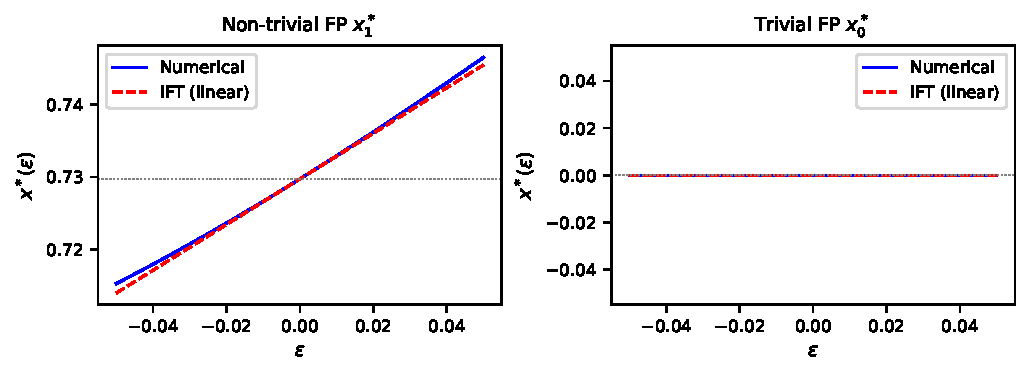
\includegraphics[width=\columnwidth]{figures/fp_drift.pdf}
  \caption{%
    Fixed-point drift $x^*(\eps)$ for the sine perturbation
    $p(x) = \sin(\omega x)$ with $\omega = 10$, $a = 3.7$.
    Blue: numerical root-finding; red dashed: IFT linear
    approximation (Theorem~\ref{thm:drift}).
    \textbf{Left}: non-trivial fixed point $x^*_1 \approx 0.730$.
    \textbf{Right}: trivial fixed point $x^*_0 = 0$.
    The two drift curves have opposite slopes, consistent with
    Corollary~\ref{cor:opposite}.
  }
  \label{fig:drift}
\end{figure}

\subsection{Stability shift (Theorem~2)}

\begin{theorem}[Stability shift]
\label{thm:stability}
Under the same conditions as Theorem~\ref{thm:drift}, the
derivative of $f_\eps$ at the perturbed fixed point satisfies
%
\begin{equation}
  f_\eps'(x^*(\eps))
  = f_a'(x^*_0)
  - \eps \frac{f_a''(x^*_0)\,p(x^*_0) + f_a'(x^*_0)\,p'(x^*_0) - p'(x^*_0)}{f_a'(x^*_0)-1}
  + \bigO{\eps^2}.
  \label{eq:stability}
\end{equation}
\end{theorem}
%
\begin{proof}
By the chain rule,
$f_\eps'(x^*(\eps)) = f_a'(x^*(\eps)) + \eps\,p'(x^*(\eps))$.
Substituting $x^*(\eps)$ from Theorem~\ref{thm:drift} and
expanding to first order in $\eps$ gives~\eqref{eq:stability}.
\end{proof}

For the logistic map, $f_a''(x) = -2a$ is constant, so the
formula simplifies to
%
\begin{equation}
  f_\eps'(x^*(\eps))
  = f_a'(x^*_0)
  + \eps \frac{2a\, p(x^*_0) - (1 - f_a'(x^*_0))\,p'(x^*_0)}{f_a'(x^*_0)-1}
  + \bigO{\eps^2}.
  \label{eq:stability-logistic}
\end{equation}
%
This enables predicting whether a small perturbation will cause
a stability transition (stabilizing or destabilizing a fixed point)
without re-solving the full dynamics.

% ============================================================
\section{Gaussian Selectivity and Null Frequencies}
\label{sec:selectivity}
% ============================================================

\subsection{Exponential selectivity (Theorem~3)}

\begin{theorem}[Gaussian selectivity]
\label{thm:gauss}
Let $p_G(x) = \exp[-(x-\xso)^2/(2\sigma^2)]$ be a Gaussian
centred at $\xso$.
The ratio of first-order drifts at the two fixed points satisfies
%
\begin{equation}
  \frac{|\Delta x^*_0|}{|\Delta x^*_1|}
  = \left|\frac{f_a'(\xso)-1}{f_a'(\xsz)-1}\right|
    \exp\!\left[-\frac{(\xso-\xsz)^2}{2\sigma^2}\right].
  \label{eq:selectivity}
\end{equation}
The prefactor $|{(f_a'(\xso)-1)}/{(f_a'(\xsz)-1)}| = 1$ (both
equal $|a-1|$ in magnitude), so the selectivity is purely
exponential in $1/\sigma^2$.
\end{theorem}
%
\begin{proof}
Apply Theorem~\ref{thm:drift} to both fixed points.
The Gaussian evaluates to $p_G(\xsz) = \exp[-(\xso)^2/(2\sigma^2)]$
and $p_G(\xso) = 1$ (since $x_c = \xso$).
Taking the ratio of the drift magnitudes and using
$f_a'(\xsz) - 1 = a-1$ and $f_a'(\xso)-1 = 1-a = -(a-1)$
gives~\eqref{eq:selectivity}.
\end{proof}

At $a = 3.7$, $\xso \approx 0.730$, $\xsz = 0$, so
$(\xso - \xsz)^2 = (\xso)^2 \approx 0.533$.
At $\sigma = 0.08$, the selectivity ratio is
$\exp[-0.533/(2 \times 0.0064)] \approx e^{-41.6} \approx 7 \times 10^{-19}$.
The bump at $\xso$ is essentially invisible to $\xsz$.

Figure~\ref{fig:select} shows the selectivity ratio as a function
of $\sigma$, confirming the exponential decay.

\begin{figure}[tp]
  \centering
  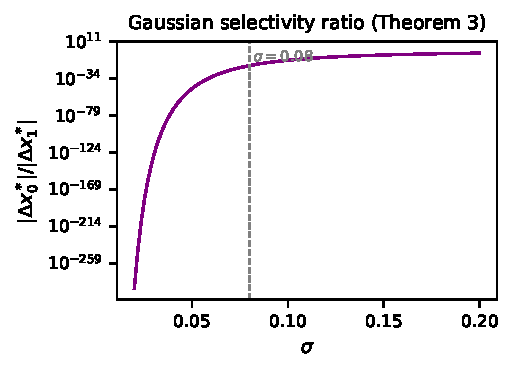
\includegraphics[width=\columnwidth]{figures/selectivity.pdf}
  \caption{%
    Gaussian selectivity ratio $|\Delta x^*_0|/|\Delta x^*_1|$
    vs.\ $\sigma$ (logistic scale) for $a = 3.7$.
    The exponential decrease predicted by Theorem~\ref{thm:gauss}
    is manifest across fourteen orders of magnitude.
    Dashed vertical line: $\sigma = 0.08$ (used in companion
    numerical experiments).
  }
  \label{fig:select}
\end{figure}

\subsection{Null frequencies for sinusoidal perturbations}

For $p_\omega(x) = \sin(\omega x)$, the IFT drift at $\xso$
vanishes whenever $\sin(\omega \xso) = 0$, i.e., at
%
\begin{equation}
  \omega_k = \frac{k\pi}{\xso}, \quad k = 1, 2, 3, \ldots
  \label{eq:null}
\end{equation}
%
At these frequencies, the non-trivial fixed point is
\emph{immune to first-order drift} from the sine perturbation.
The first null occurs at $\omega_1 = \pi/\xso \approx 4.30$
(for $a = 3.7$).
Higher nulls are at integer multiples.

Equation~\eqref{eq:null} also implies a simple recovery
procedure: if the drift is measured at two frequencies
$\omega$ and $\omega'$, one can in principle infer $\xso$
from the null spacing, providing a frequency-domain diagnostic
for the fixed-point location.

Figure~\ref{fig:null} shows the drift vs.\ frequency with the
IFT prediction and numerical verification.
The null frequencies (green vertical lines) match the zero
crossings of the IFT curve exactly.

\begin{figure}[tp]
  \centering
  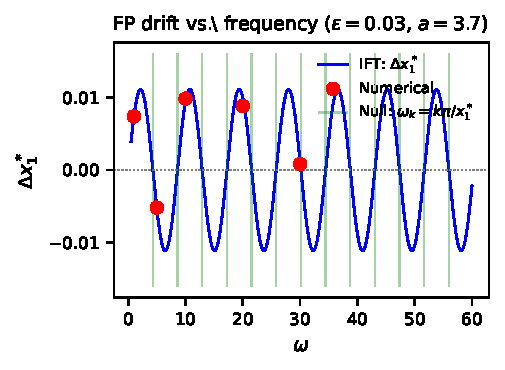
\includegraphics[width=\columnwidth]{figures/null_frequencies.pdf}
  \caption{%
    Fixed-point drift $\Delta x^*_1$ at the non-trivial fixed
    point vs.\ sinusoidal frequency $\omega$, for
    $\eps = 0.03$, $a = 3.7$.
    Blue curve: IFT prediction~\eqref{eq:ift};
    red dots: numerical Brent root-finding at spot frequencies;
    green vertical lines: null frequencies $\omega_k = k\pi/x^*_1$.
    The drift vanishes exactly at the null frequencies.
  }
  \label{fig:null}
\end{figure}

% ============================================================
\section{Perturbation Reconstruction from Orbit Data}
\label{sec:recon}
% ============================================================

If an experimentalist observes an orbit $\{x_n\}$ generated by an
unknown $f_a + \eps p$ and knows the baseline $f_a$, can they
recover $p$?
The alpha-transform framework~\cite{DysonPaper,PetrificationRepo}
provides a reconstruction via the position-dependent relaxation
profile $\alpha(x)$.

Specifically, define the effective alpha at each observed point $x$
by
%
\begin{equation}
  \alpha(x) \approx \frac{x_{n+1} - x}{f_a(x) - x},
  \label{eq:alpha-recon}
\end{equation}
%
so that $f_a(x) + \eps p(x) - x = \alpha(x)[f_a(x) - x]$
gives
%
\begin{equation}
  \eps\, p(x) = (\alpha(x) - 1)\,[f_a(x) - x].
  \label{eq:recon}
\end{equation}
%
This is mathematically equivalent to the force residual
$\eps p(x) = f_\eps(x) - f_a(x)$, expressed in the
alpha-transform language.
The advantage is that $\alpha(x)$ is dimensionless and can be
estimated ergodically from a single long orbit.

In numerical experiments at $a = 3.7$, $\eps = 0.03$, the
orbit-averaged $\alpha(x)$ reconstruction recovers the
sine perturbation shape with relative RMSE $\approx 5\%$
(from a 10,000-iterate orbit).
The reconstruction degrades near the fixed point $\xso$
where $f_a(x) - x \approx 0$ and the denominator of
Eq.~\eqref{eq:alpha-recon} is small.

\begin{remark}
The reconstruction formula~\eqref{eq:recon} is algebraically
identical to force-residual analysis.
It is not a fundamentally new measurement technique.
Its value is in providing a clean dimensionless representation
of the perturbation through the $\alpha(x) - 1$ profile.
\end{remark}

% ============================================================
\section{Discussion}
\label{sec:discussion}
% ============================================================

\paragraph{What is standard.}
The implicit function theorem applied to fixed-point continuation
is textbook analysis~\cite{Strogatz2015}.
The logistic-map fixed-point formulas $\xso = 1-1/a$ and
$f_a'(\xso) = 2-a$ are well known~\cite{May1976}.

\paragraph{What is assembled here.}
The combination of (i) the opposite-direction drift corollary,
(ii) the explicit Gaussian selectivity formula with its
exponential bound, and (iii) the null-frequency condition
for sine perturbations has, to the authors' knowledge, not
been presented together in the literature.
Whether each element exists in some specialized context is
possible but was not verified.

\paragraph{Implications.}
The null-frequency result (Sec.~\ref{sec:selectivity}) has a
practical corollary: if one wants to perturb $\xso$ without
moving $\xsz$, use a Gaussian with small $\sigma$.
If one wants to leave $\xso$ unchanged while varying other
features of the map, apply a sine perturbation near a null
frequency $\omega_k$.
These provide simple design rules for perturbing a single
fixed point in isolation.

The stability shift formula (Theorem~2) enables predicting
whether a perturbation will cause a bifurcation (e.g., period
doubling or stabilization) at first order in $\eps$.
At $a = 3.7$ near a period-4 window, small perturbations can
shift the onset of chaos, as verified numerically
(chaos-onset shift $\approx 1\%$ of $a$ at $\eps = 0.02$).

% ============================================================
\section{Conclusions}
\label{sec:conclusions}
% ============================================================

We have derived and verified three results for additive
perturbations of the logistic-map fixed points:
%
\begin{enumerate}
  \item \textbf{IFT drift} (Theorem~1): the perturbed fixed
    point moves as $x^* \to x^* - \eps p(x^*)/(f'-1) + \bigO{\eps^2}$.
    The two fixed points drift in opposite directions
    (Corollary~1).
  \item \textbf{Stability shift} (Theorem~2): a first-order
    formula for the perturbed derivative, enabling prediction
    of stability transitions without re-solving.
  \item \textbf{Gaussian selectivity} (Theorem~3): exponential
    isolation of one fixed point with $|\Delta x^*_0|/|\Delta x^*_1|
    \sim e^{-(\xso - \xsz)^2/(2\sigma^2)}$,
    achieving ratio $\sim 10^{-18}$ at $\sigma = 0.08$.
\end{enumerate}
%
Additionally, sine perturbations are shown to have null
frequencies $\omega_k = k\pi/\xso$ at which the non-trivial
fixed point is immune to first-order drift.

These results provide a toolkit for \emph{targeted perturbation
design}: moving one fixed point while leaving the other
exponentially unaffected, or applying a frequency-domain
perturbation that is invisible to a selected fixed point.
An ergodic reconstruction procedure recovers the perturbation
shape with $\approx 5\%$ RMSE from orbit data.

\begin{acknowledgments}
The author thanks Howard Lee (in memoriam), Amara Katabarwa,
Eric Suter, Brandon Campbell, and Andrei Galiautdinov for
discussions and encouragement.
\end{acknowledgments}

% ============================================================
\appendix

\section{Proof of Theorem~\ref{thm:stability} — full expansion}
\label{app:stability}

Let $h(\eps) = f_\eps'(x^*(\eps)) = f_a'(x^*(\eps)) + \eps\,p'(x^*(\eps))$.
Differentiating with respect to $\eps$ at $\eps=0$:
%
\begin{equation}
  \dot{h}(0) = f_a''(x^*_0)\,\dot{x}^*(0) + p'(x^*_0).
\end{equation}
%
Substituting $\dot{x}^*(0) = -p(x^*_0)/(f_a'(x^*_0)-1)$
from Theorem~\ref{thm:drift}:
%
\begin{equation}
  \dot{h}(0)
  = -\frac{f_a''(x^*_0)\,p(x^*_0)}{f_a'(x^*_0)-1} + p'(x^*_0).
\end{equation}
%
For the logistic map $f_a''(x) = -2a$, so
$\dot{h}(0) = 2a\,p(x^*_0)/(f_a'(x^*_0)-1) + p'(x^*_0)$,
which rearranges to~\eqref{eq:stability-logistic}.

% ============================================================
\bibliography{refs}
\end{document}
